\chapter{Deployment}

Das Front- und Backend sollen auf einem Linux Server deployed werden. Im Folgenden soll das Aufsetzen des Servers, der Domain sowie die Inbetriebnahme der beiden Anwendungen näher erläutert werden.

\section{Bereitstellen des Linux Servers und der Domain}

Zuerst muss ein Linux Server bereitgestellt werden, auf dem später das Front- und Backend betrieben werden sollen. Für diese Studienarbeit wird hierfür ein \ac{VPS} der Firma netcup empfohlen. Die \acp{VPS} von netcup bieten unter Anderem eine stundenbasierte Abrechnung, DDoS-Schutz, eine Mindestverfügbarkeit von 99,6 \% pro Jahr sowie SSD Festplatten mit RAID10. Der angebotene \ac{VPS} 200 mit einem CPU-Kern, 2GB RAM und 20GB Speicher für monatlich 2,69 € \cite[vgl.][]{NetcupVPS} ist für diese Studienarbeit ausreichend.

Der \ac{VPS} kann unter \cite{NetcupVPS} bestellt werden. Sollte noch keine Domain existieren, kann diese ebenfalls bei netcup für 5€ pro Jahr (für eine .de Domain) unter \cite{NetcupDomains} bestellt werden.

\subsection{Installation von Ubuntu}
Sobald der \ac{VPS} von netcup bereitgestellt wurde, soll Ubuntu als Betriebssystem installiert werden. Standardmäßig wird der Server mit Debian vorinstalliert.

Dazu muss sich unter \lstinline{https://www.servercontrolpanel.de/SCP/Home} in die Verwaltungsoberfläche des \ac{VPS} angemeldet werden. Anschließend kann wie in Abbildung \ref{fig:netcup-ubuntu-installation} zu sehen, ein neues Betriebssystem unter dem Menüpunkt \glqq Medien\grqq{} installiert werden. Hier sollte die aktuellste Version von Ubuntu ausgewählt und die folgenden Installationsschritte durchgeführt werden.

\begin{figure}[H]
  \setlength{\fboxsep}{0pt}
  \setlength{\fboxrule}{0.5pt}
  \fbox{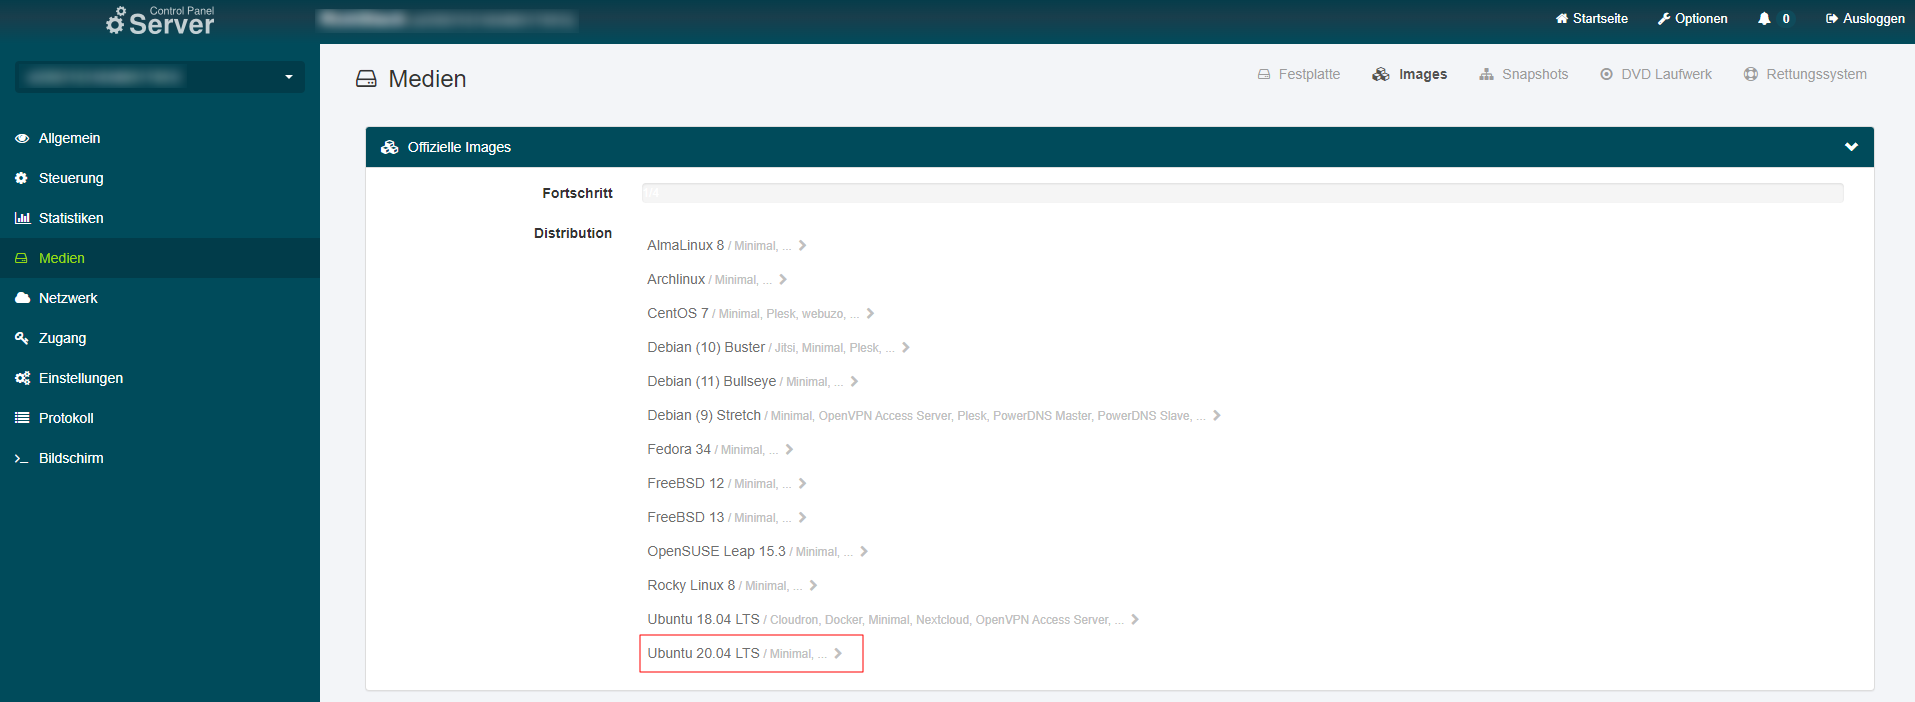
\includegraphics[width=0.9\textwidth]{images/netcup-ubuntu-installation.png}}
  \centering
  \caption[Installation von Ubuntu auf dem VPS]{Installation von Ubuntu auf dem VPS}
  \label{fig:netcup-ubuntu-installation}
\end{figure}

\subsection{Zugriff auf den VPS / Einrichtung eines SSH-Clients}
Für einen benutzerfreundlichen Zugriff auf den \ac{VPS} wird die Entwicklungsumgebung \ac{VS Code} empfohlen. Nach der Installation mithilfe von \cite{VSCode} muss die \glqq Remote - SSH\grqq{} Erweiterung installiert werden (siehe Abbildung \ref{fig:vscode-remote-ssh}).

\begin{figure}[H]
  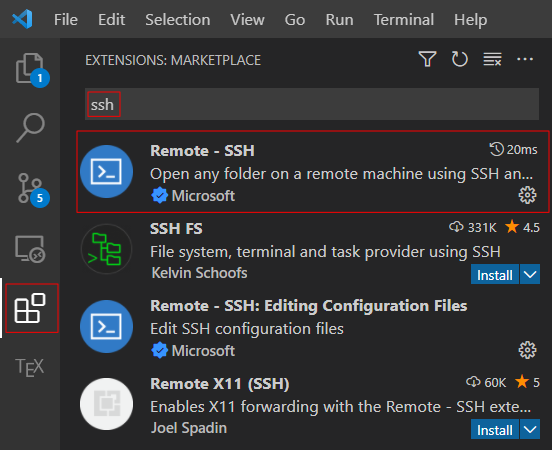
\includegraphics[width=0.75\textwidth]{images/vscode-remote-ssh.png}
  \centering
  \caption[Einrichtung von VS Code als SSH-Client]{Einrichtung von VS Code als SSH-Client}
  \label{fig:vscode-remote-ssh}
\end{figure}

Sobald die Erweiterung installiert ist, befindet sich in \ac{VS Code} unten links ein grünes Symbol, über das eine Verbindung mit dem \ac{VPS} hergestellt werden kann. Dazu muss auf das Symbol geklickt und in dem sich öffnendem Auswahlmenü \glqq Connect to Host\grqq{} ausgewählt werden. Anschließend muss angegeben werden mit welchem Host (Server) sich verbunden werden soll. Dazu muss \lstinline{root@VPS_IP} eingegeben werden, wobei \lstinline{VPS_IP} durch die IP-Adresse des \ac{VPS} ersetzt werden muss. Diese findet sich in der E-Mail Bestätigung von netcup oder in der Verwaltungsoberfläche unter dem Menüpunkt \glqq Netzwerk\grqq{}. Das Passwort für den Zugriff befindet sich ebenfalls in der E-Mail Bestätigung oder auf der Verwaltungsoberfläche nach Installation von Ubuntu.

Nach erfolgreicher Verbindung können mit \ac{VS Code} über die Benutzeroberfläche Dateien/Ordner erstellt und geöffnet bzw. bearbeitet werden.

\subsection{Konfiguration der Domain / DNS}
Sobald die bestellte Domain von netcup bereitgestellt wurde, müssen die DNS Einstellungen der Domain geändert werden, damit sie auf die IP-Adresse des \ac{VPS} zeigt.

Dazu muss sich unter \lstinline{https://www.customercontrolpanel.de/} in das Kundenkonto angemeldet werden. Anschließend ist unter dem Menüpunkt \glqq Domains\grqq{} die bestellte Domain aufgelistet. Durch einen Klick auf das Lupen-Symbol lassen sich die DNS-Einstellungen der Domain anpassen.

\begin{figure}[H]
  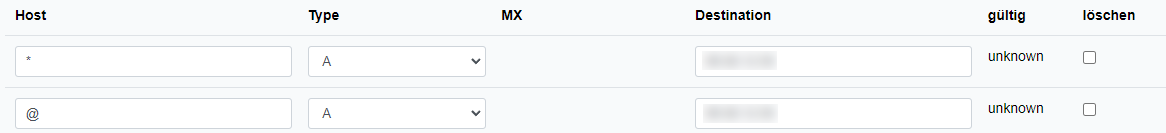
\includegraphics[width=0.9\textwidth]{images/netcup-dns.png}
  \centering
  \caption[Einrichtung der Domain]{Einrichtung der Domain}
  \label{fig:netcup-dns}
\end{figure}

Die DNS-Einträge müssen mindestens so wie in Abbildung \ref{fig:netcup-dns} konfiguriert werden, wobei als Destination die IP-Adresse des \ac{VPS} eingetragen werden muss. Beim Aufruf der Domain in z.B. einem Browser führt diese nun auf den \ac{VPS}. Die Änderungen der DNS-Einstellungen kann bis zu 48 Stunden dauern. In der Regel sind diese jedoch bereits nach einigen Minuten aktiv.

\section{Einrichtung des nginx-proxy}
Nun ist der \ac{VPS} und die Domain erfolgreich eingerichtet. Im Folgenden wird erläutert, wie das Front- und Backend eingerichtet werden können, damit über die Domain auch auf die Anwendungen zugegriffen werden kann und diese nicht ins leere führt.

Die Anwendungen werden als Docker Container gestartet. Basierend auf dem Docker Container \lstinline{nginx-proxy} von jwilder werden die Anwendungen (Front- und Backend) dann über die Domain erreichbar gemacht und automatisch SSL-Zertifikate angefragt und verwaltet, damit die Daten per \lstinline{https} verschlüsselt sind. Auf Docker und docker-compose wird im Rahmen dieser Studienarbeit nicht weiter eingegangen.

\subsection{Installation von Docker und docker-compose}
Da sowohl der nginx-proxy, als auch das Front-und Backend mit Docker betrieben werden sollen, muss Docker und docker-compose installiert werden. Installationsanleitungen können entsprechend auf \cite{DockerInstallation} und \cite{DockerDomposeInstallation} gefunden werden.

Um die Installation zu vereinfachen, kann auch das Skript unter \lstinline{https://github.com/larsrickert/nginx-proxy/blob/main/utils/install-docker-ubuntu.sh} verwendet werden. Es beinhaltet die offiziellen Installationsschritte zur Installation der aktuellsten Versionen von Docker und docker-compose.

Dazu muss die genannte Datei auf den \ac{VPS} kopiert werden und das Skript mit

\begin{center}
  \lstinline{bash ./install-docker-ubuntu.sh}
\end{center}

ausgeführt werden.

\subsection{Installation des nginx-proxy}
Nach der Installation von Docker und docker-compose muss der nginx-proxy selbst installiert werden. Dazu kann die Installationsanleitung unter \cite{NginxProxyInstallation} (\lstinline{https://nginxproxy.lars-rickert.de/guide/getting-started.html}) verwendet werden.

Der nginx-proxy ist dafür zuständig, jede Docker-Anwendung, die die Umgebungsvariablen \lstinline{VIRTUAL_HOST} und \lstinline{LETSENCRYPT_HOST} gesetzt hat, über ebendiesen host/Domain zur Verfügung zu stellen. Dabei verwaltet er automatisch SSL-Zertifikate von Let's Encrypt, um die Verbindung über SSL zu verschlüsseln \cite{NginxProxyDeployment}. Dies ist für das Front- und Backend bereits in der \lstinline{docker-compose.yml} realisiert, sodass lediglich die Domain in der \lstinline{.env} Datei eingetragen werden muss (siehe Kapitel \ref{sec:start-applications}).

\section{Starten des Front- und Backends}
\label{sec:start-applications}
Um nun das Front- und Backend dieser Studienarbeit bereitzustellen, muss zuerst mit

\begin{center}
  \lstinline{git clone https://github.com/philippabele/nursing-home-volunteer.git}
\end{center}

der Code von GitHub heruntergeladen werden.

Danach muss die Datei \lstinline{.env.example} kopiert und in \lstinline{.env} umbenannt werden. Diese Datei enthält alle sensiblen Umgebungsvariablen für den Betrieb der beiden Anwendungen. Diese sollten niemals öffentlich geteilt werden. Nach dem Anlegen der \lstinline{.env} Datei sollten die Werte der Umgebungsvariablen entsprechend geändert werden.

Nun kann das Front- und Backend durch

\begin{center}
  \lstinline{docker-compose up -d}
\end{center}

gestartet werden. Der zuvor eingerichtete nginx-proxy erkennt die beiden Anwendungen automatisch und stellt sie entsprechend über die \lstinline{FRONTEND_DOMAIN} und \lstinline{BACKEND_DOMAIN} bereit, die in der \lstinline{.env} Datei eingetragen wurden. Es sei angemerkt, dass die Anforderung der SSL-Zertifikate für die Domains ein paar Sekunden dauern kann, sodass direkt nach dem Starten eine Fehlermeldung des Browser erscheinen kann, dass die SSL-Zertifikate nicht gültig sind.

Sollten neue Änderungen für die Anwendungen verfügbar, d.h. der Code auf GitHub geändert worden sein, können sie mit

\begin{center}
  \lstinline{git pull && docker-compose up -d --build}
\end{center}

aktualisiert werden.

\section{Datensicherung und Umzug auf einen anderen Server}
Sollte der Bedarf für eine vollständige Datensicherung der Anwendungen bestehen oder diese z.B. auf einen anderen \ac{VPS} umgezogen werden sollen, ist dies durch die Verwendung von Docker benutzerfreundlich möglich.

Um die Daten der beiden Anwendungen vollständig zu sichern, muss lediglich der Order \lstinline{docker-data} und die Datei \lstinline{.env} gesichert werden. \lstinline{docker-data} wird hierbei beim Start der Anwendungen mit docker-compose erstellt und persistiert die Datenbank des Backends sowie alle hochgeladenen Medien. Das Frontend besteht lediglich aus statischen kompilierten Dateien, sodass dieses nicht gesichert werden muss.

Bei einem Umzug auf einen anderen \ac{VPS} muss die in diesem Kapitel beschriebene Einrichtung des Servers (inkl. Docker, docker-compose und nginx-proxy) sowie der Domain durchgeführt werden. Anschließend können die gesicherten Daten (\lstinline{docker-data} und \lstinline{.env}) auf den neuen Server kopiert und die Anwendungen, wie in Kapitel \ref{sec:start-applications} beschrieben, gestartet werden.
